\documentclass{beamer}

\usetheme{Madrid}
\usepackage[utf8]{inputenc}
\usepackage{default}
\usepackage{default}

\usepackage{soul}
\makeatletter
\newcommand\SoulColor{%
  \let\set@color\beamerorig@set@color
  \let\reset@color\beamerorig@reset@color}
\makeatother

\newcommand*\MyPitem{%
  \item[\color{green}\scalebox{0.9}{\textbullet}]}
\newcommand*\MyCitem{%
  \item[\color{red}\scalebox{0.9}{\textbullet}]}

\AtBeginSection[]
{
\begin{frame}<beamer>
\frametitle{Outline}
\tableofcontents[currentsection]
\end{frame}
}

\begin{document}

\section{Motivation}

%PART 1 : Motivation
\begin{frame}{Motivation}

    \begin{figure}
    \centering
    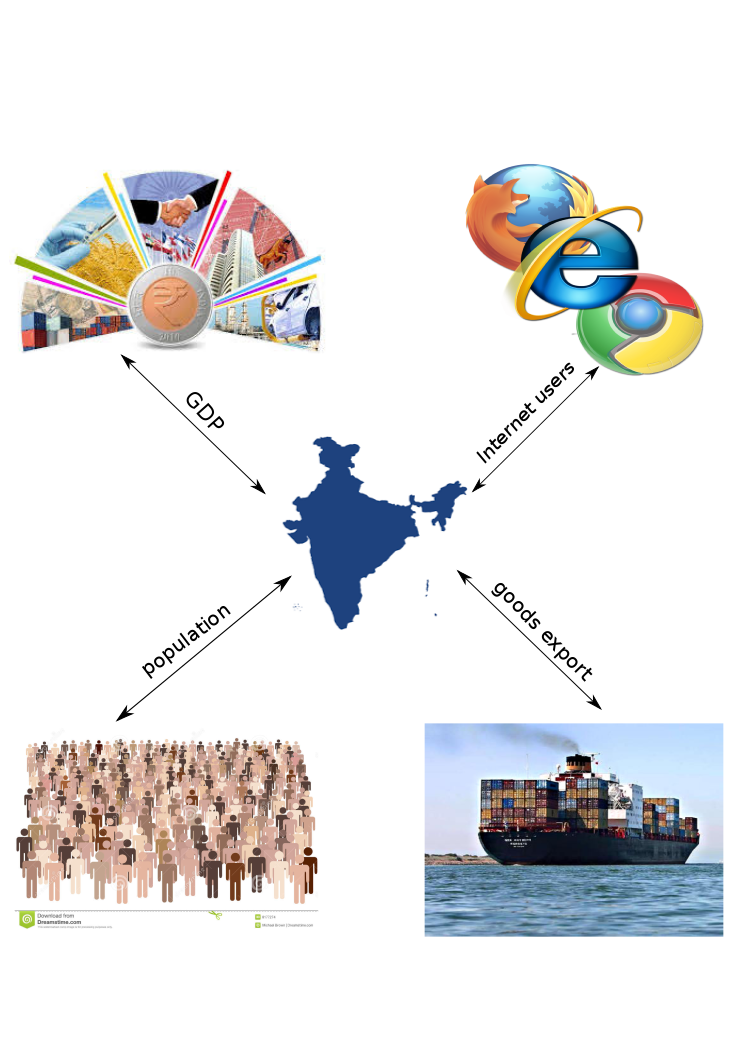
\includegraphics[width = 0.5\textwidth]{images/motivation}
  \end{figure}
 
\end{frame}
\begin{frame}{Motivation}
 
 \begin{itemize}
  \item Repositories of facts containing this information can be found at many places, like data.worldbank.org, Wikipedia infoboxes etc. \pause
  \item Countries are popular and finite, finding complete knowledge bases is possible. \pause
  \item What about less popular entities?  \pause
    \begin{itemize}
      \item What is the population of Arbit Apartments, Powai? \pause
      \item What is the GDP of Sugarcane Industry of India? \pause
      \item Percent of Internet users in Mumbai? 
    \end{itemize}
 \end{itemize} 
\end{frame}
\begin{frame}{Motivation}

\begin{itemize}
 \item  Good News!!! \pause
 \item  Web is huge, probably, there is some page which contains the information we are looking for. \pause
 \item The way in which you express a fact about an entity depends on the fact, and not the entity. \pause
 \item We may expect the sentence structure to be similar. \pause
 \begin{itemize}
    \item Population of India reached 1.3 billion, making it the second largest country in the world
    \item Population of Arbit Apartments, Powai reached 1300
 \end{itemize}
 
\end{itemize}
\end{frame}

\section{Problem Statement}
\begin{frame}{Problem Statement}
 \begin{itemize}
  \item Given that we know a lot about countries, can we train extractors that run over the web and pull similar facts about other entities?
 \end{itemize}
\end{frame}
\begin{frame}{Introduction}

\begin{itemize}
 
 \item  The knowledge is scattered in unstructured text on the web.
 
  \begin{figure}
    \centering
    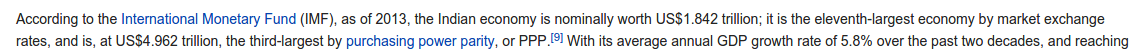
\includegraphics[width = 1.0\textwidth]{images/ex_1}
  \end{figure}
  
  \begin{figure}
    \centering
    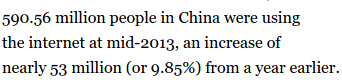
\includegraphics[width = 0.3\textwidth]{images/ex_2}
  \end{figure}
  
    \begin{figure}
    \centering
    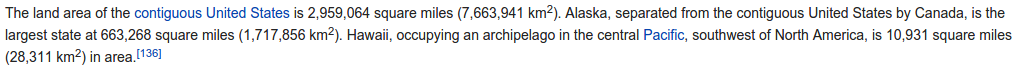
\includegraphics[width = 1.0\textwidth]{images/ex_3}
  \end{figure}
  

  \item Can such facts be extracted automatically?
\end{itemize}

\end{frame}
\begin{frame}{Relation Extraction: Problem}
\begin{itemize}
 \item Extract 3-tuples which consists of an entity and a numerical value that are bound by some relation.
  
    \begin{itemize}
	\item  (India, \textbf{economy}, 1.842 trillion USD)
	\item  (China, \textbf{internet users},  590.56 million)
	\item  (USA, \textbf{land area}, 2,959,054 square mile)
    \end{itemize}

 \end{itemize}
\end{frame}

%PART 2 : Relation extraction as a machine learning problem

\section{Relation Extractions as a Machine Learning Problem}
\begin{frame}
\begin{block}{Relation extraction as a Machine Learning Problem}
\end{block}
\end{frame}
\begin{frame}{Machine Learning for Relation Extraction}
 \begin{itemize}
  \item Structure and content of sentences expressing the same relations can be expected to be similar. 
 \begin{itemize}
      \item The population of Australia is estimated to be 23,622,400 as of 7 October 2014.
      \item According to an official estimate for 1 June 2014, the population of Russia is 143,800,000.   
   \end{itemize}   
 \end{itemize}
\end{frame}
\begin{frame}{Machine Learning for Relation Extraction}
\begin{itemize}
\item  Structure and content of sentences expressing the same relations can be expected to be similar. 
 \begin{itemize}   
    \item At 17,075,400 square kilometres, Russia is the largest country in the world.
    \item With an area of 504,030 $km^{2}$, Spain is the second largest country in Western Europe.
    \end{itemize}
 \end{itemize}
\end{frame}
\begin{frame}{Machine Learning for Relation Extraction}
 
 \begin{itemize}
  \item Redundancy in grammatical features and dependencies of the sentences expressing same relation. \pause
     \begin{figure}
    \centering
    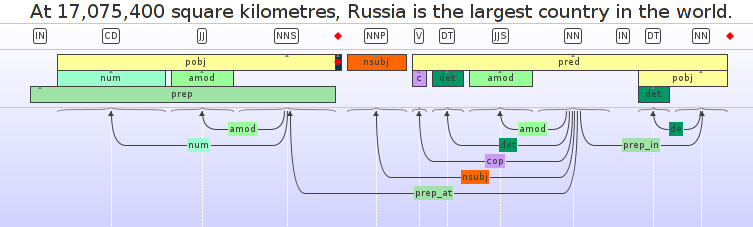
\includegraphics[width = 0.8\textwidth]{images/ex_4}
  \end{figure} \pause
  
   \begin{figure}
    \centering
    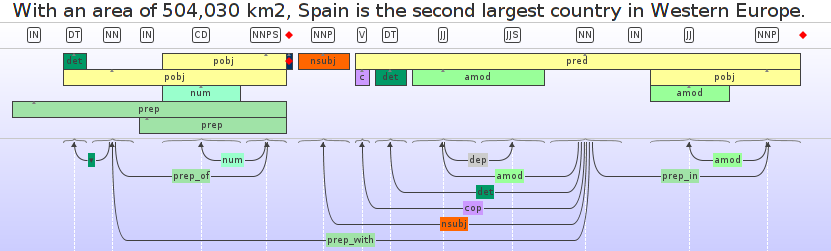
\includegraphics[width = 0.8\textwidth]{images/ex_5}
  \end{figure}
 \end{itemize}

\end{frame}
\begin{frame}{Machine Learning for Relation Extraction}
\begin{itemize}
  \item There is lot of redundancy in ways in which a relation is expressed in sentence. \pause
  \item So for every relation learn the patterns that express it. \pause
    \begin{itemize}
      \item grammatical patterns - POS tags, dependency parse. \pause
      \item keywords for the relations. \pause
    \end{itemize}
    
    \item This forms the relation extraction as a multi-class classification problem.
 \end{itemize}
\end{frame}
\begin{frame}{Possible Workflow}
  \begin{itemize}
   \item Collect enough examples for each relation so that there are sufficient patterns and enough redundancy to exploit.
   \item Extract features (important keywords, grammatical structure, parse tress, etc.) for these sentences.
   \item Learn a multi-class classifier on this training data (Explained later).
   \item Once the model is learnt, for every sentence 
    \begin{itemize}
	\item Extract features for the sentence
	\item Predict the relation using the model for these features
	\item store the fact into database.
     \end{itemize}
  \end{itemize}
\end{frame}
\begin{frame}{Challenge}
 \begin{itemize}
  \item The size of corpus is enormous (e.g, 5 million sentences).  \pause
  \item It is very hard to go through the entire corpus and label each sentence to one of the relations. \pause
  \item For model to generalize well, we need lot of training data. \pause
  \item What to do then?
 \end{itemize}
\end{frame}

\section{Distant Supervision}
%PART 3 DS
\begin{frame}{Distant Supervision}
\begin{itemize}
 \item Manual labeling of the entire corpus is not possible
 \item Weak Supervision as a middle ground
  \item Use Heuristics to align a table of facts with the corpus
  \item Fuzzy training 
  
\end{itemize}
\end{frame}
\begin{frame}{Distant Supervision}{Example}
\begin{itemize}
 
\item Born - In database
 \begin{center}
\begin{tabular}{|l|l|}
\hline
Donald Knuth & Wisconsin \\
Srinivasa Ramanujan & Erode \\
Alan Turing & London \\
\hline
\end{tabular}
\end{center}
\item Given Sentences
\begin{itemize}
\item Srinivasa Ramanujan was born in his maternal grandmother’s home in Erode.
\item Srinivasa Ramanujan was born in Erode, Tamilnadu, India, on 22nd December, 1887.
\item Turing was born in Paddington, London, while his father was on leave from his position with the Indian Civil Service (ICS) at Chhatrapur, Bihar
\item Alan Turing biopic The Imitation Game named as London film festival opener.
\end{itemize}
\end{itemize}
 
\end{frame}
\begin{frame}{Distant Supervision}{Example}
\begin{itemize}
 
\item Born - In database
 \begin{center}
\begin{tabular}{|l|l|}
\hline
Donald Knuth & Wisconsin \\
\SoulColor\hl{Srinivasa Ramanujan} & \SoulColor\hl{Erode} \\
Alan Turing & London \\
\hline
\end{tabular}
\end{center}
\item Given Sentences
\setbeamercolor{normal text}{fg=gray,bg=}
\setbeamercolor{alerted text}{fg=black,bg=}
\usebeamercolor{normal text}
\begin{itemize}
\item \alert<+> {\SoulColor\hl{Srinivasa Ramanujan} was born in his maternal grandmother’s home in \SoulColor\hl{Erode}.} \alert{LABEL : BornIn}
\item Srinivasa Ramanujan was born in Erode, Tamilnadu, India, on 22nd December, 1887.
\item Turing was born in Paddington, London, while his father was on leave from his position with the Indian Civil Service (ICS) at Chhatrapur, Bihar
\item Alan Turing biopic The Imitation Game named as London film festival opener.
\end{itemize}
\end{itemize}
 
\end{frame}
\begin{frame}{Distant Supervision}{Example}
\begin{itemize}
 
\item Born - In database
 \begin{center}
\begin{tabular}{|l|l|}
\hline
Donald Knuth & Wisconsin \\
\SoulColor\hl{Srinivasa Ramanujan} & \SoulColor\hl{Erode} \\
Alan Turing & London \\
\hline
\end{tabular}
\end{center}
\item Given Sentences
\setbeamercolor{normal text}{fg=gray,bg=}
\setbeamercolor{alerted text}{fg=black,bg=}
\usebeamercolor{normal text}
\begin{itemize}
\item Srinivasa Ramanujan was born in his maternal grandmother’s home in Erode.
\item \alert<+> {\SoulColor\hl{Srinivasa Ramanujan} was born in \SoulColor\hl{Erode}, Tamilnadu, India, on 22nd December, 1887.}
\item Turing was born in Paddington, London, while his father was on leave from his position with the Indian Civil Service (ICS) at Chhatrapur, Bihar
\item Alan Turing biopic The Imitation Game named as London film festival opener.
\end{itemize}
\end{itemize}
 
\end{frame}
\begin{frame}{Distant Supervision}{Example}
\begin{itemize}
 
\item Born - In database
 \begin{center}
\begin{tabular}{|l|l|}
\hline
Donald Knuth & Wisconsin \\
Srinivasa Ramanujan & Erode \\
\SoulColor\hl{Alan Turing} & \SoulColor\hl{London} \\
\hline
\end{tabular}
\end{center}
\item Given Sentences
\setbeamercolor{normal text}{fg=gray,bg=}
\setbeamercolor{alerted text}{fg=black,bg=}
\usebeamercolor{normal text}
\begin{itemize}
\item Srinivasa Ramanujan was born in his maternal grandmother’s home in Erode.
\item Srinivasa Ramanujan was born in Erode, Tamilnadu, India, on 22nd December, 1887.
\item \alert<+> {\SoulColor\hl{Turing} was born in Paddington, \SoulColor\hl{London}, while his father was on leave from his position with the Indian Civil Service (ICS) at Chhatrapur, Bihar}
\item Alan Turing biopic The Imitation Game named as London film festival opener.
\end{itemize}
\end{itemize}
 
\end{frame}
\begin{frame}{Distant Supervision}{Example}
\begin{itemize}
 
\item Born - In database
 \begin{center}
\begin{tabular}{|l|l|}
\hline
Donald Knuth & Wisconsin \\
Srinivasa Ramanujan & Erode \\
\SoulColor\hl{Alan Turing} & \SoulColor\hl{London} \\
\hline
\end{tabular}
\end{center}
\item Given Sentences
\setbeamercolor{normal text}{fg=gray,bg=}
\setbeamercolor{alerted text}{fg=black,bg=}
\usebeamercolor{normal text}
\begin{itemize}
\item Srinivasa Ramanujan was born in his maternal grandmother’s home in Erode.
\item Srinivasa Ramanujan was born in Erode, Tamilnadu, India, on 22nd December, 1887.
\item Turing was born in Paddington, London, while his father was on leave from his position with the Indian Civil Service (ICS) at Chhatrapur, Bihar
\item \alert<+> {\SoulColor\hl{Alan Turing} biopic The Imitation Game named as \SoulColor\hl{London} film festival opener.}
\end{itemize}
\end{itemize}
 
\end{frame}
\begin{frame}{Distant Supervision}
\begin{itemize}
\item[\textcolor{red}{$\bullet$}] Distant supervision assumption, any sentence containing the entity pair will express the corresponding relation
\item[\textcolor{green}{$\bullet$}] Can quickly label huge corpora
\item[\textcolor{red}{$\bullet$}] Same entity pair can match different relations (Founded(Steve Jobs, Apple) or CEO(Steve Jobs, Apple))
\item[\textcolor{red}{$\bullet$}] False positives, may lead to model learning wrong patterns for relations
\end{itemize}
\end{frame}

\section{Distant Supervision Techniques}
%PART 4: MultiR
\begin{frame}{Distant Supervision Techniques}
 \begin{itemize}
  \item First paper in 1999, almost every possibility explored
 \end{itemize}
\begin{center}
 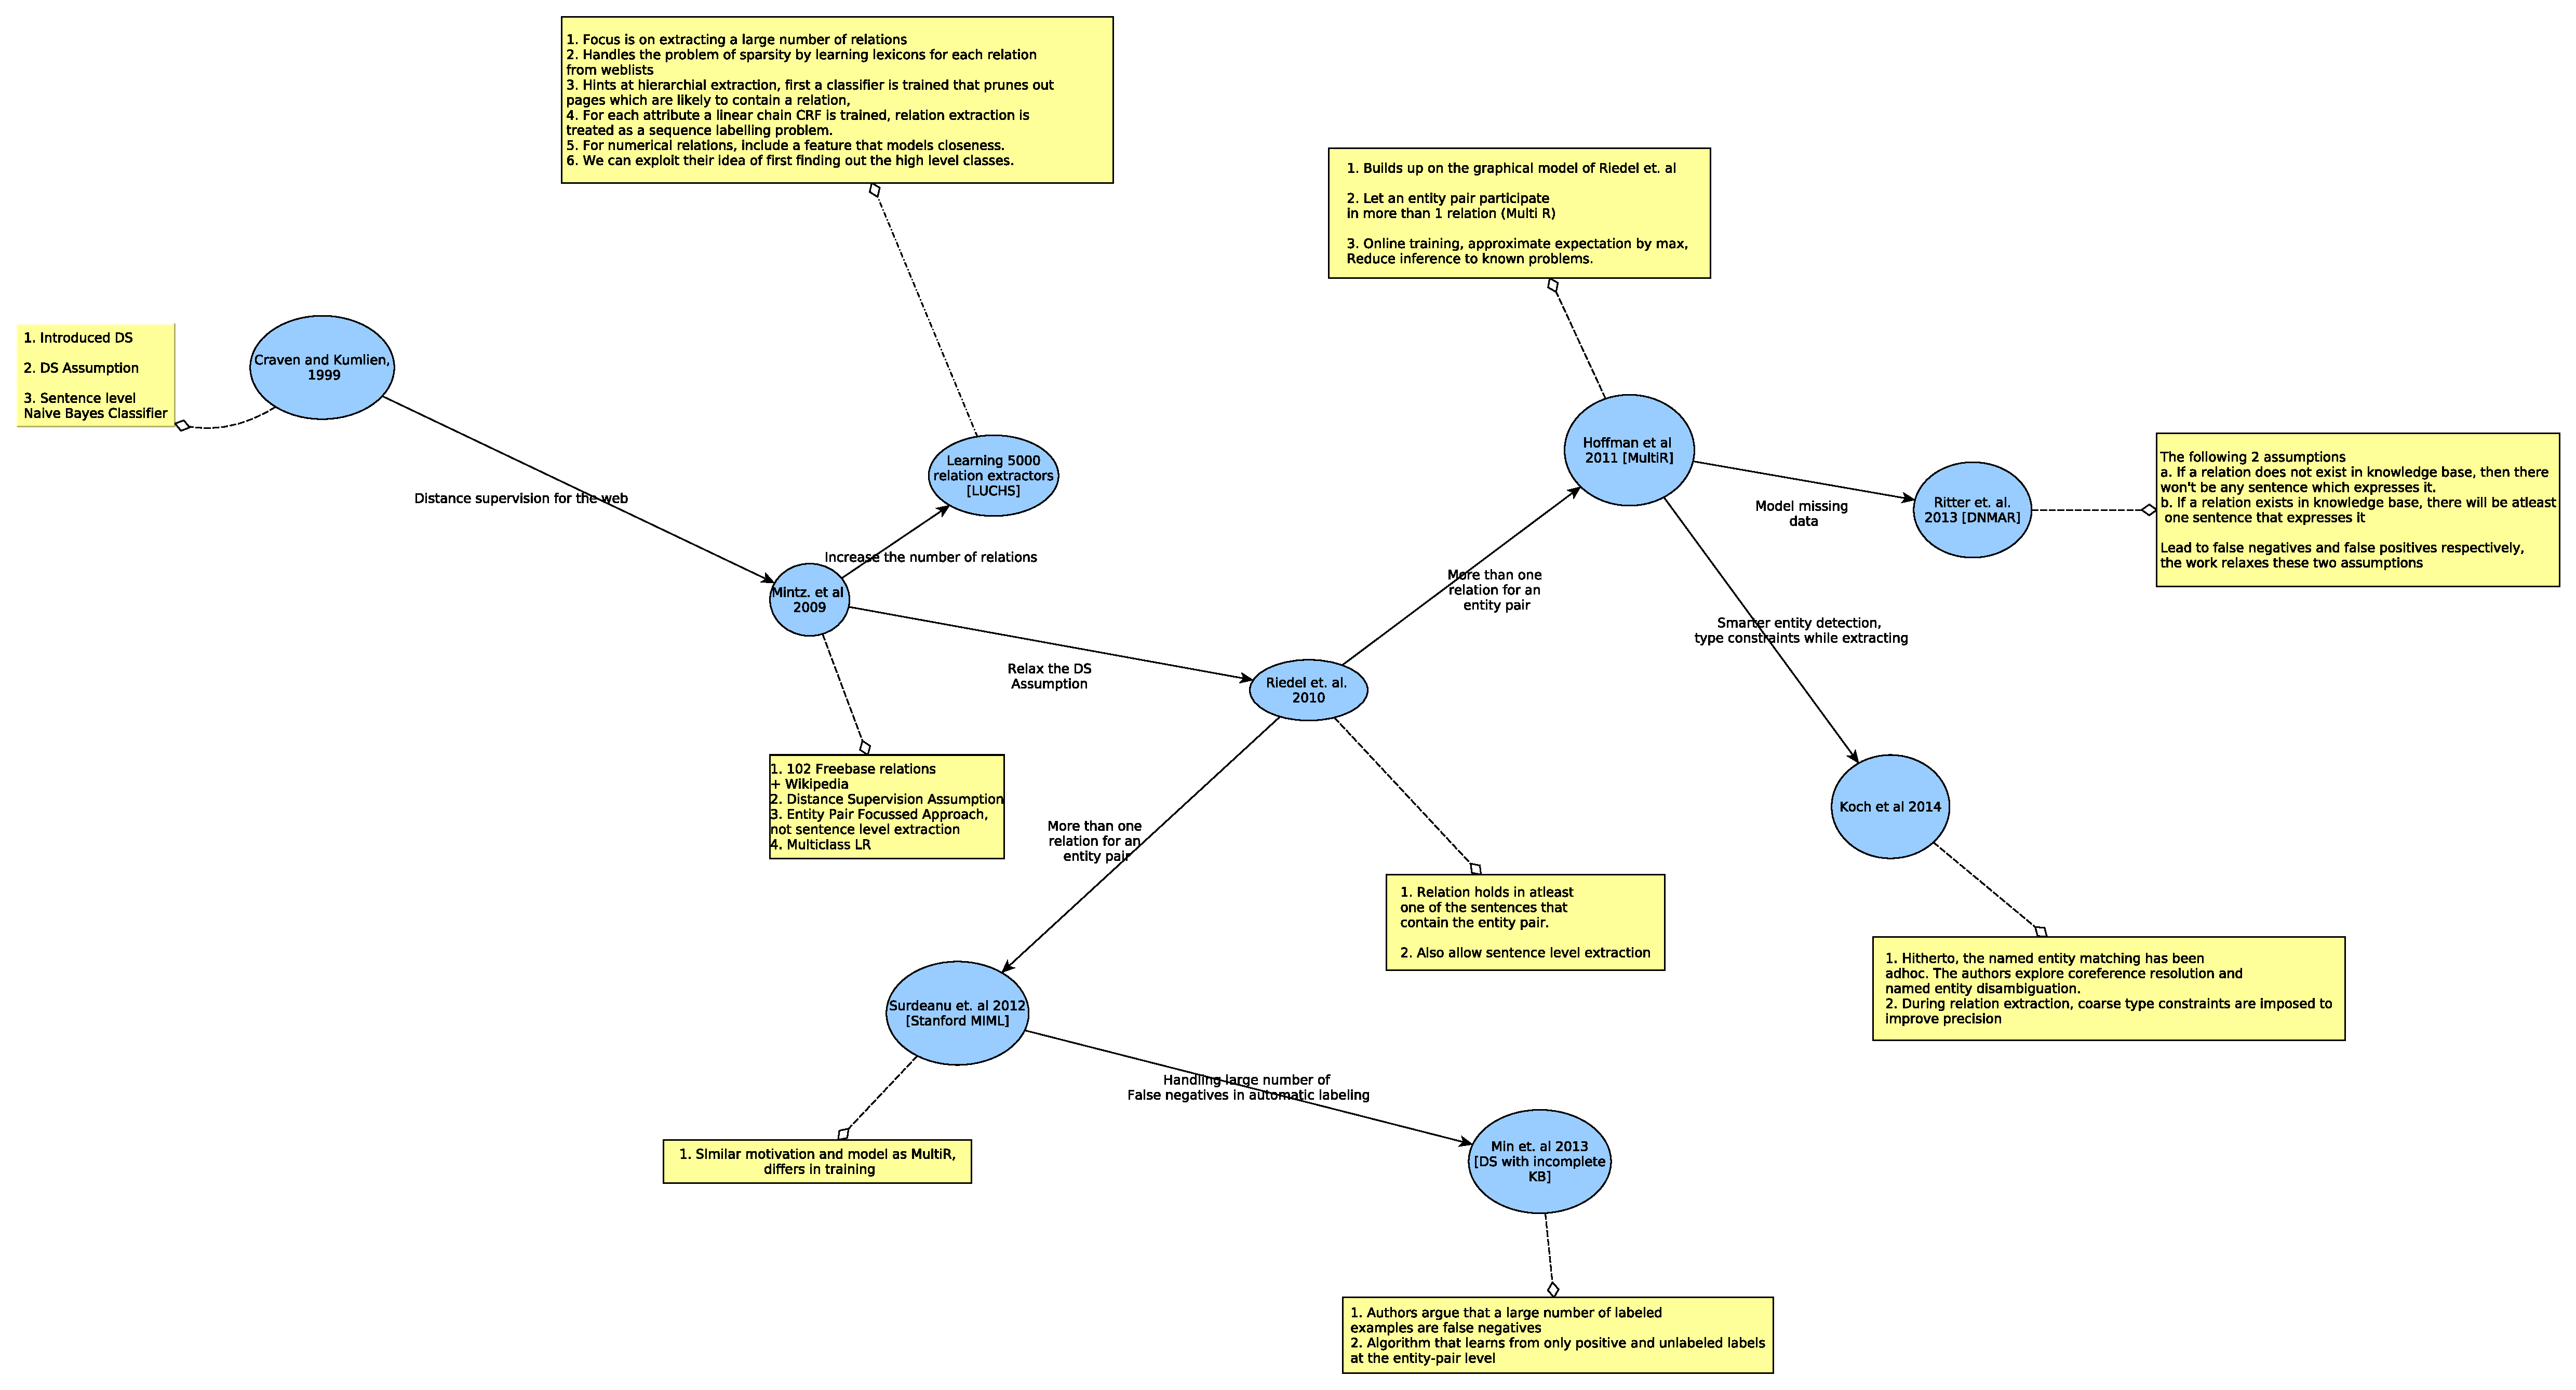
\includegraphics[scale=0.12]{./imgs/dsreadings.pdf}
 % dsreadings.pdf: 2381x1285 pixel, 72dpi, 84.00x45.33 cm, bb=0 0 2381 1285
\end{center}
\end{frame}
\begin{frame}{Distant Supervision Techniques}
 \begin{itemize}
  \item First paper in 1999, \emph{almost} every possibility explored
 \end{itemize}
\begin{center}
 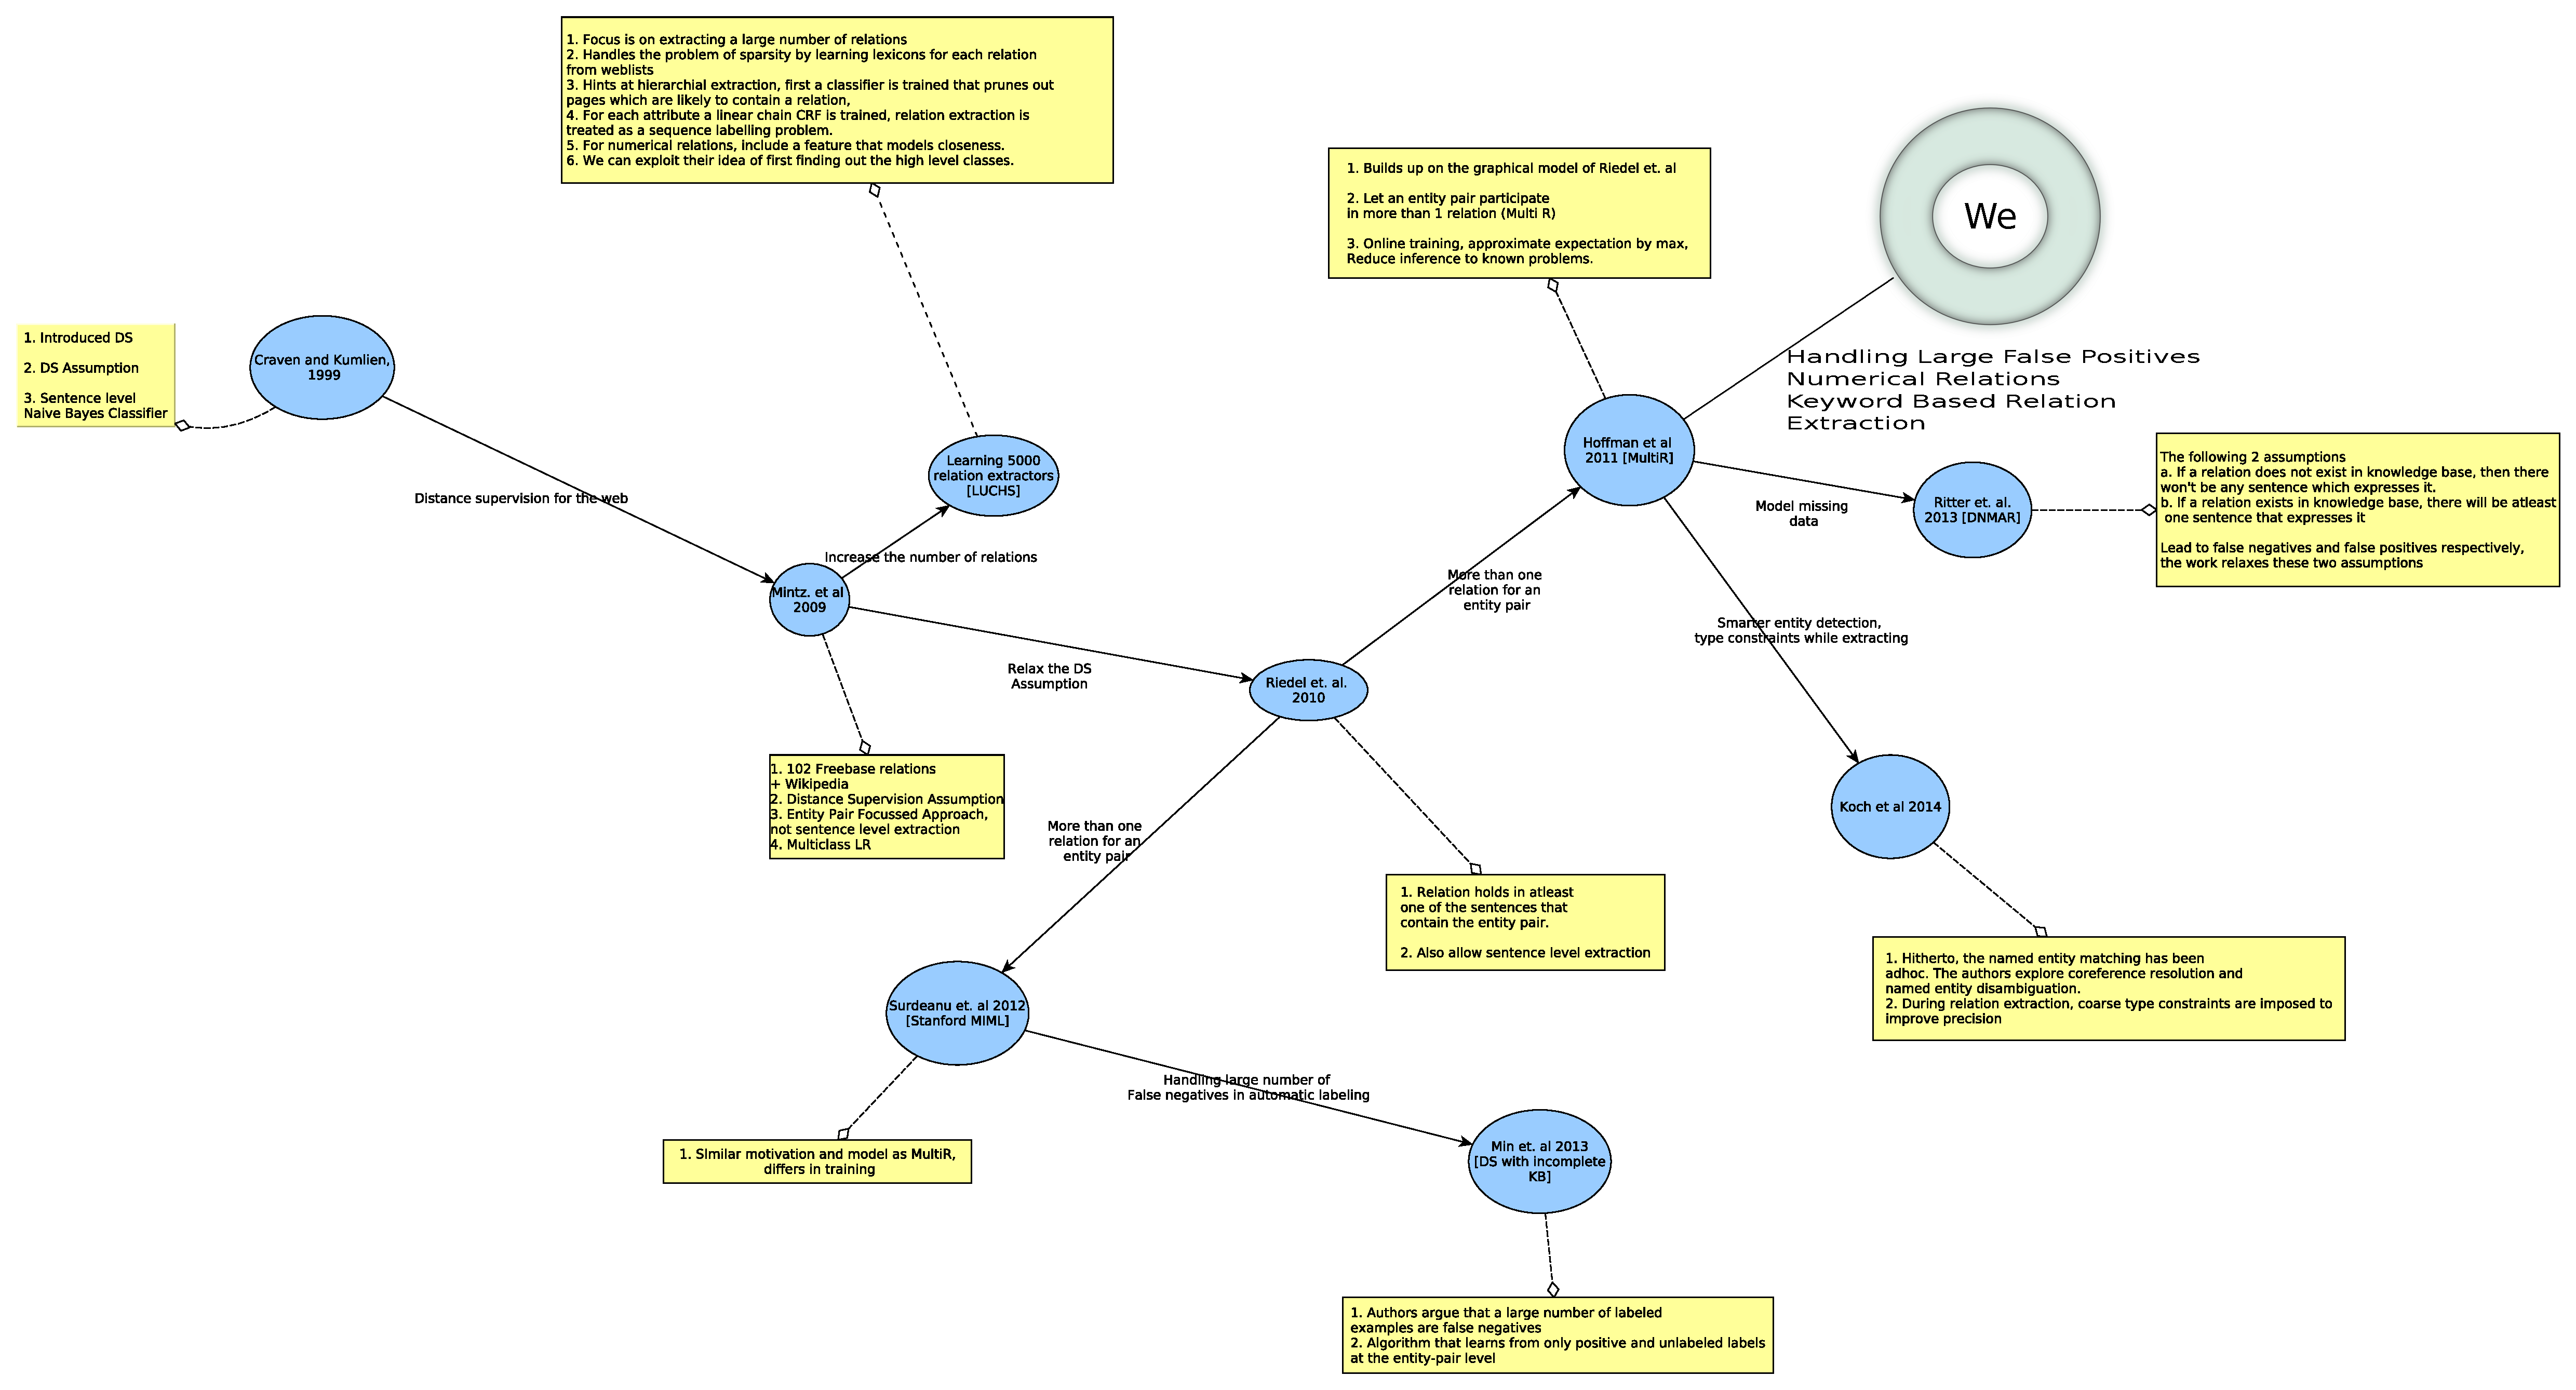
\includegraphics[scale=0.12]{./imgs/us.pdf}
 % us.pdf: 2381x1285 pixel, 72dpi, 84.00x45.33 cm, bb=0 0 2381 1285
\end{center}

\end{frame}
\begin{frame}{Relation Extraction Using MultiR}{From \url{raphaelhoffmann.com/publications}}
\begin{figure}[h]
 \centering
 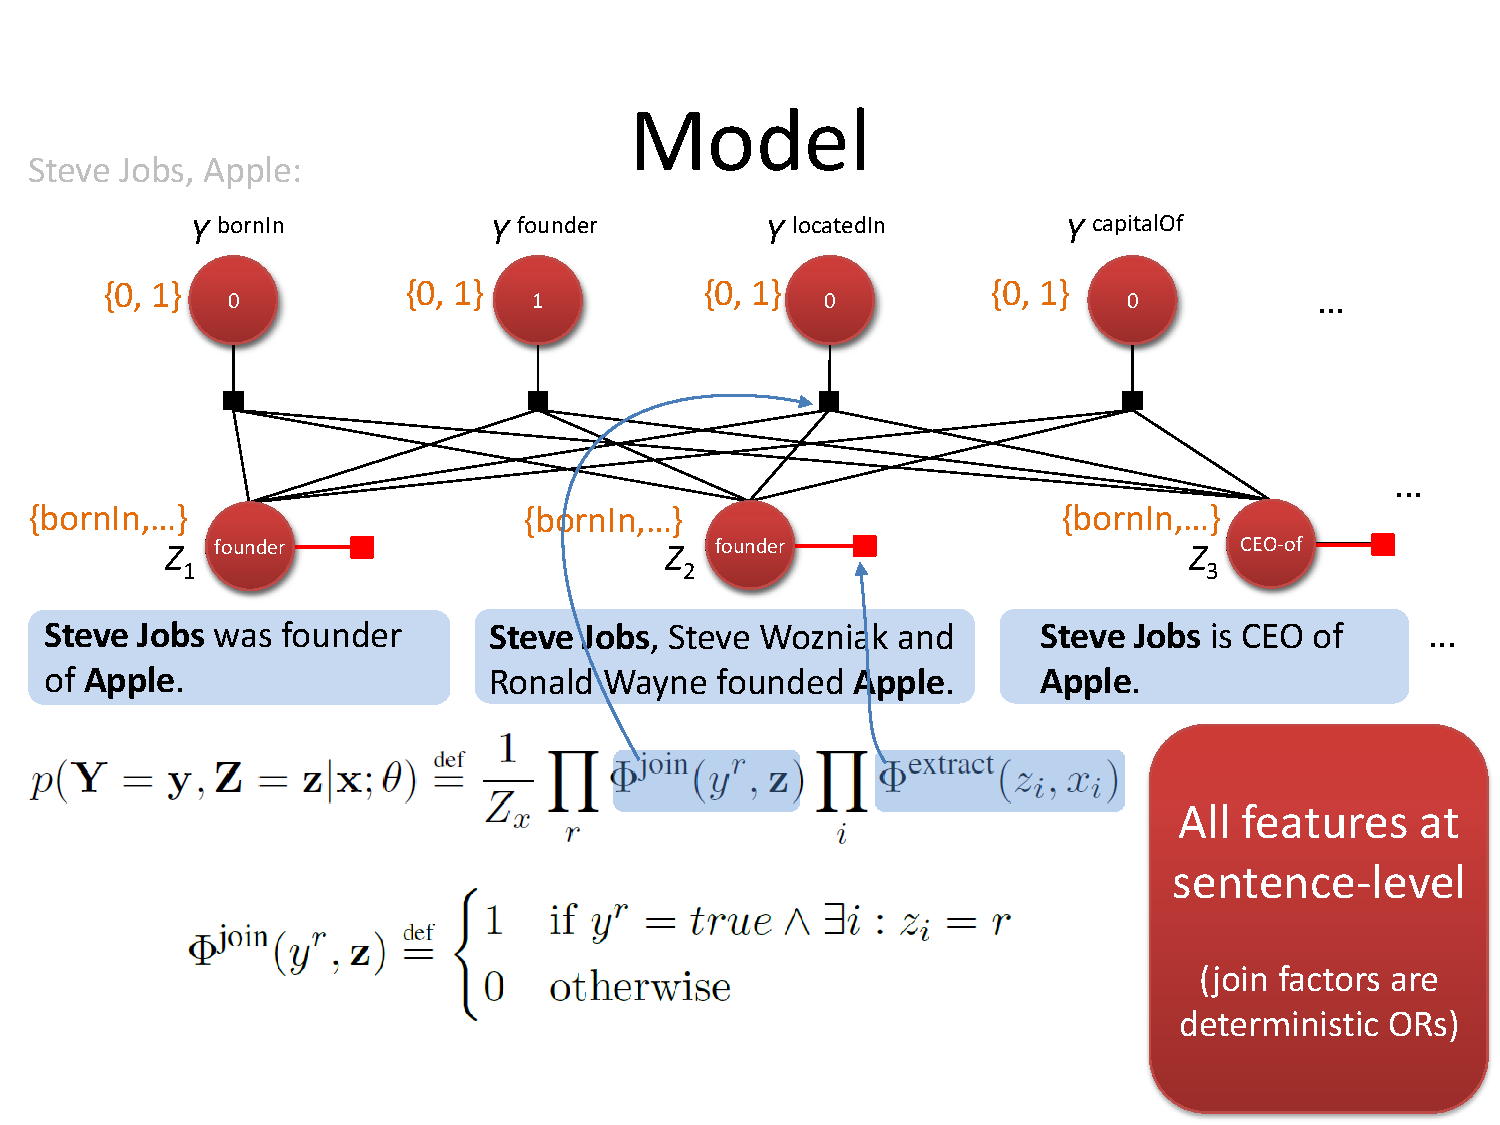
\includegraphics[scale=0.40]{./imgs/multirmode1.pdf}
 % multirmode.1.pdf: 720x540 pixel, 72dpi, 25.40x19.05 cm, bb=0 0 720 540
 \end{figure}
\end{frame}
\begin{frame}{Relation Extraction Using MultiR}{From \url{raphaelhoffmann.com/publications}}
\begin{figure}[h]
 \centering
 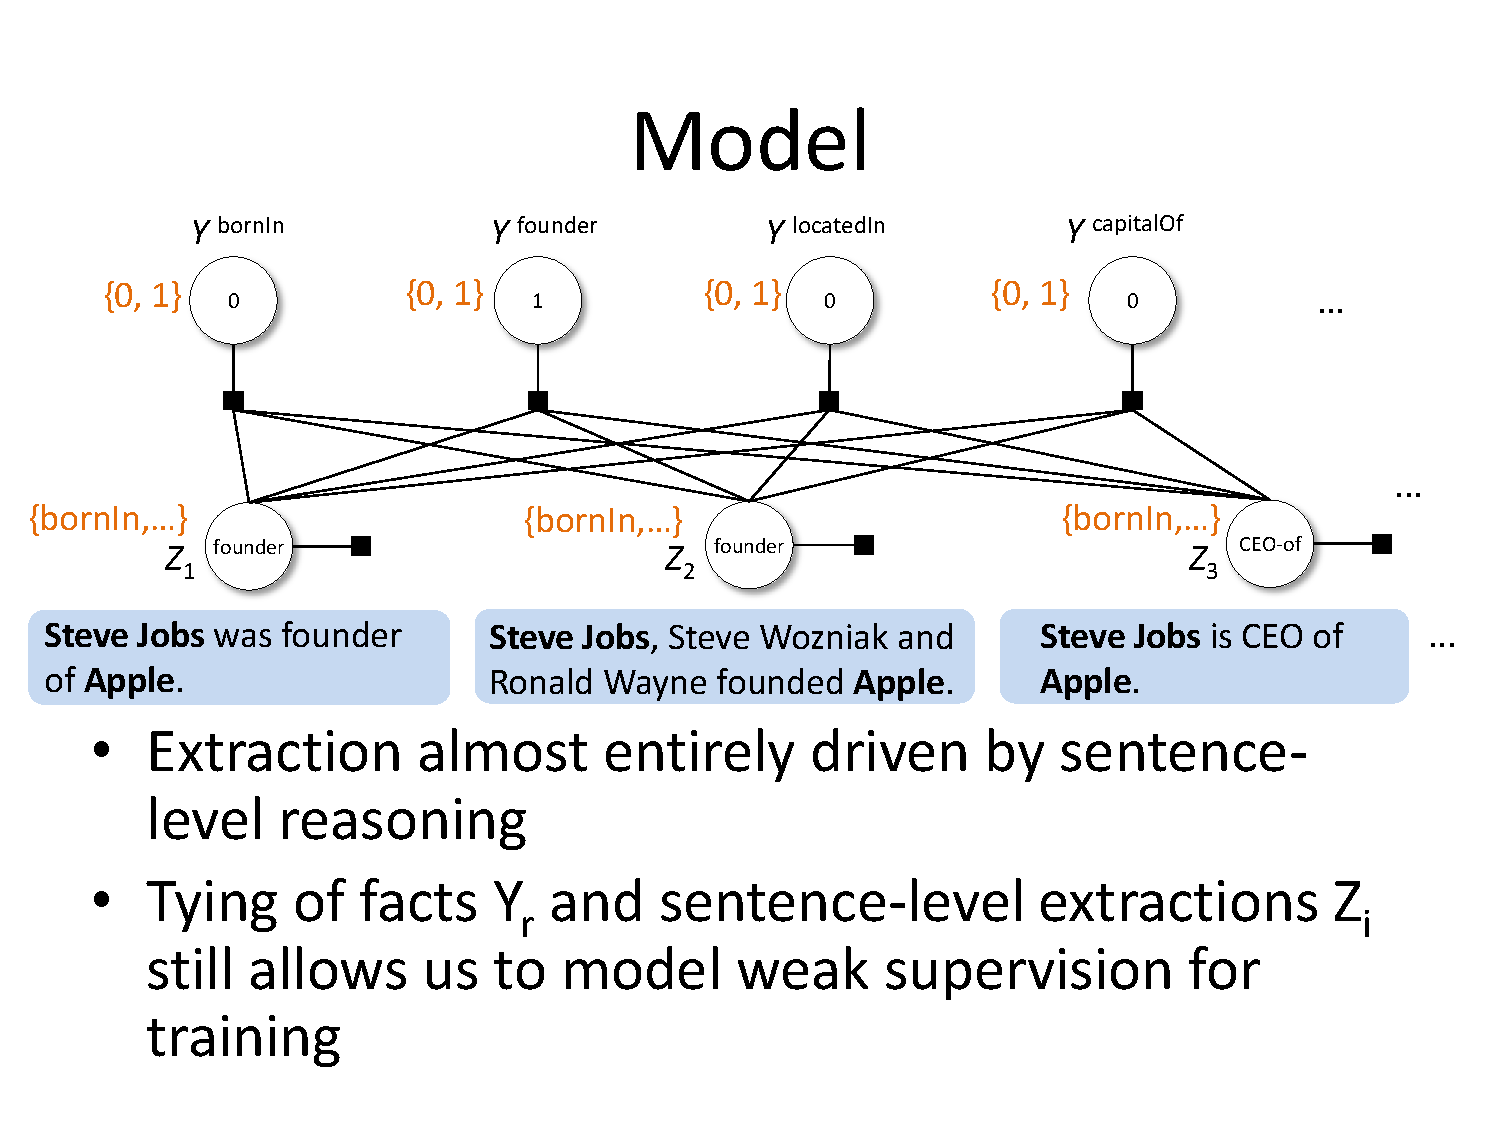
\includegraphics[scale=0.40]{./imgs/multirmode2.pdf}
 % multirmode.1.pdf: 720x540 pixel, 72dpi, 25.40x19.05 cm, bb=0 0 720 540
 \end{figure}
\end{frame}
\begin{frame}{Relation Extraction Using MultiR}{From \url{raphaelhoffmann.com/publications}}
\begin{figure}[h]
 \centering
 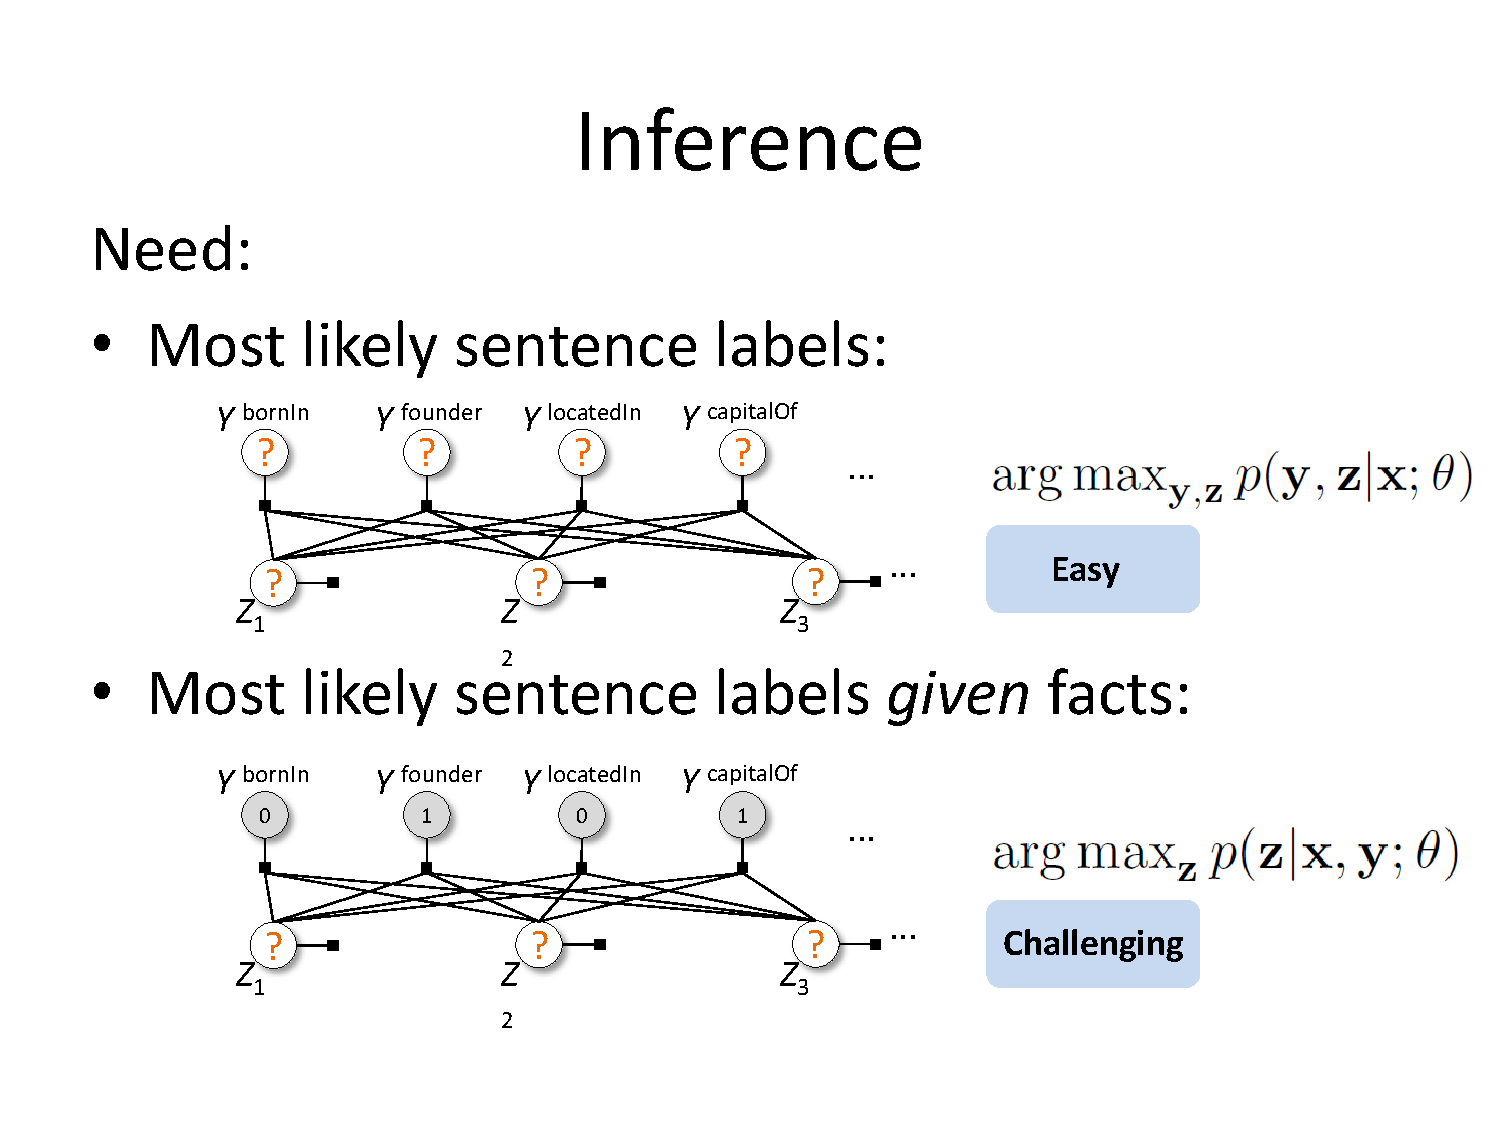
\includegraphics[scale=0.40]{./imgs/multirmode3.pdf}
 % multirmode.1.pdf: 720x540 pixel, 72dpi, 25.40x19.05 cm, bb=0 0 720 540
 \end{figure}
\end{frame}
\begin{frame}{Relation Extraction Using MultiR}{From \url{raphaelhoffmann.com/publications}}
\begin{figure}[h]
 \centering
 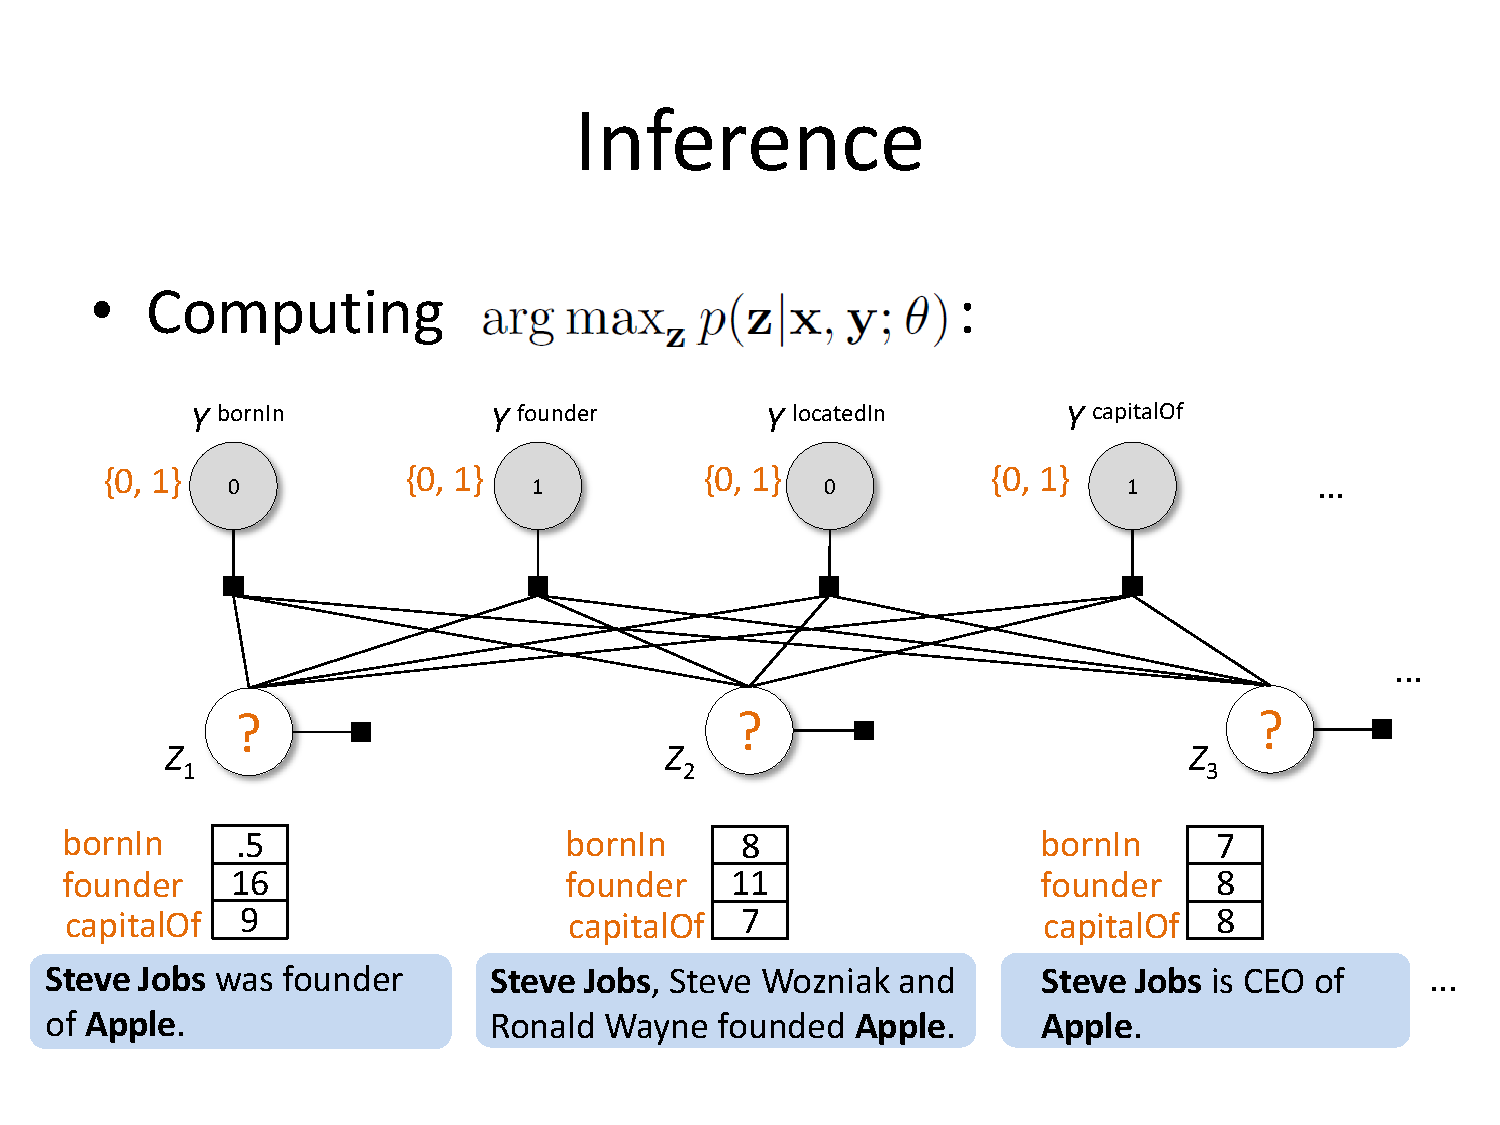
\includegraphics[scale=0.40]{./imgs/multirmode4.pdf}
 % multirmode.1.pdf: 720x540 pixel, 72dpi, 25.40x19.05 cm, bb=0 0 720 540
 \end{figure}
\end{frame}
\begin{frame}{Relation Extraction Using MultiR}{From \url{raphaelhoffmann.com/publications}}
\begin{figure}[h]
 \centering
 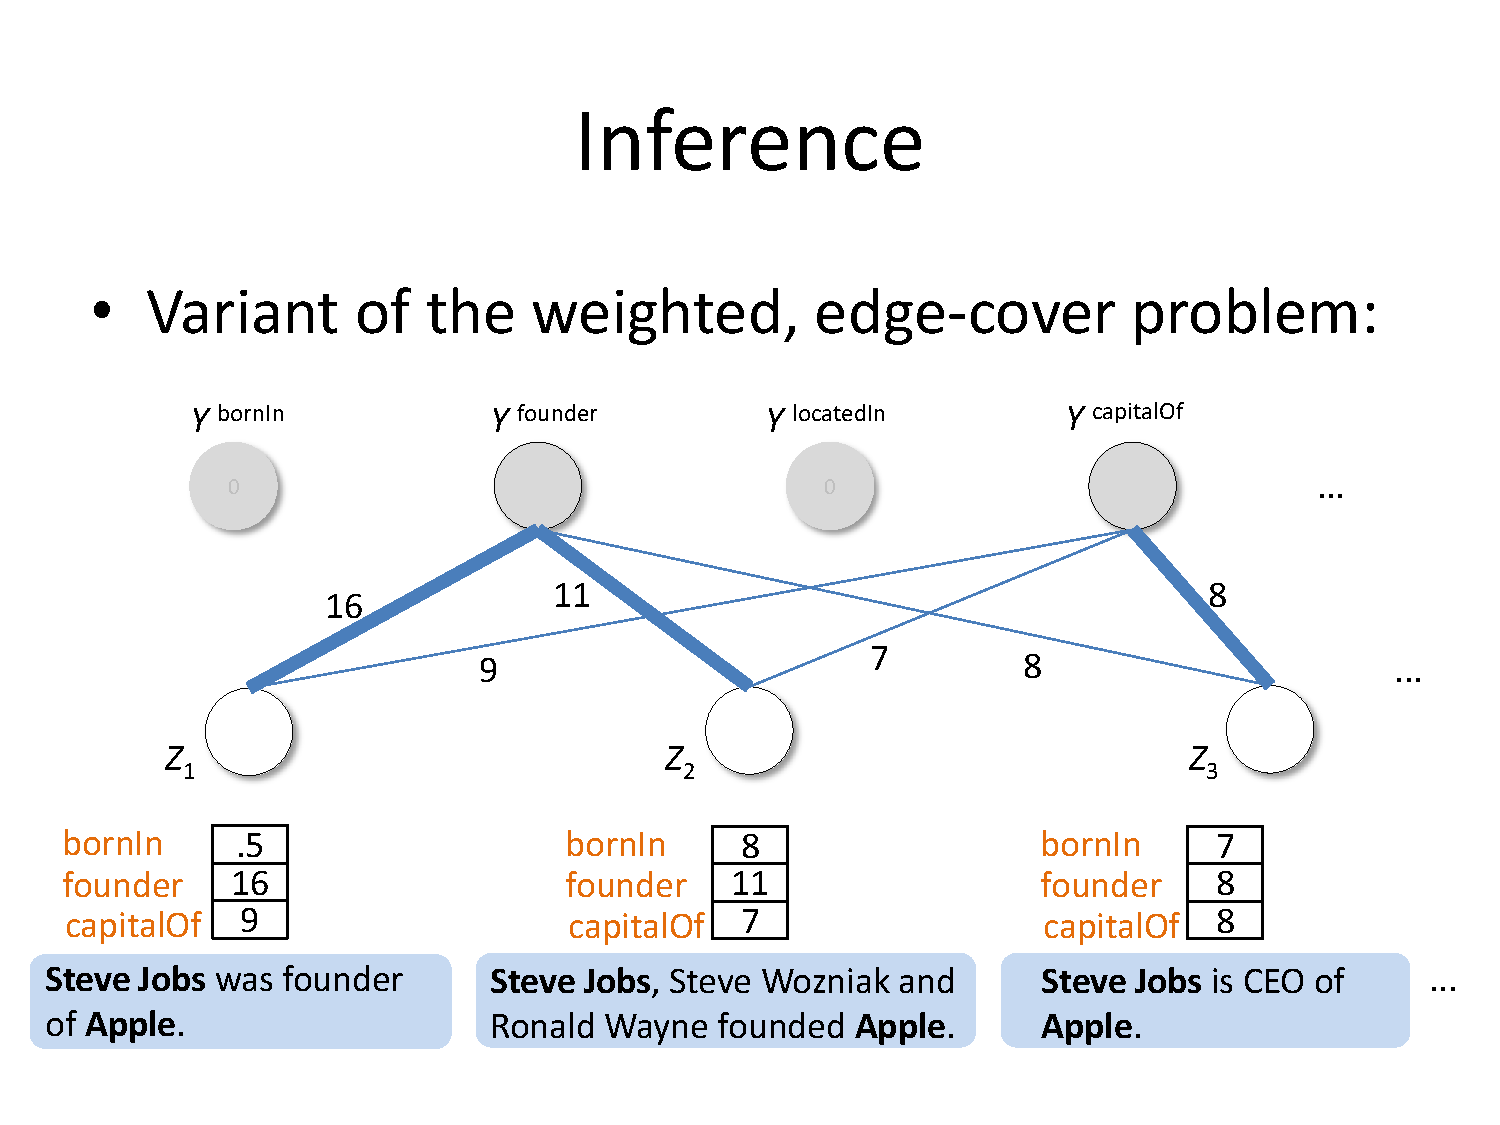
\includegraphics[scale=0.40]{./imgs/multirmode5.pdf}
 % multirmode.1.pdf: 720x540 pixel, 72dpi, 25.40x19.05 cm, bb=0 0 720 540
 \end{figure}
\end{frame}
\begin{frame}{Relation Extraction Using MultiR}{From \url{raphaelhoffmann.com/publications}}
\begin{figure}[h]
 \centering
 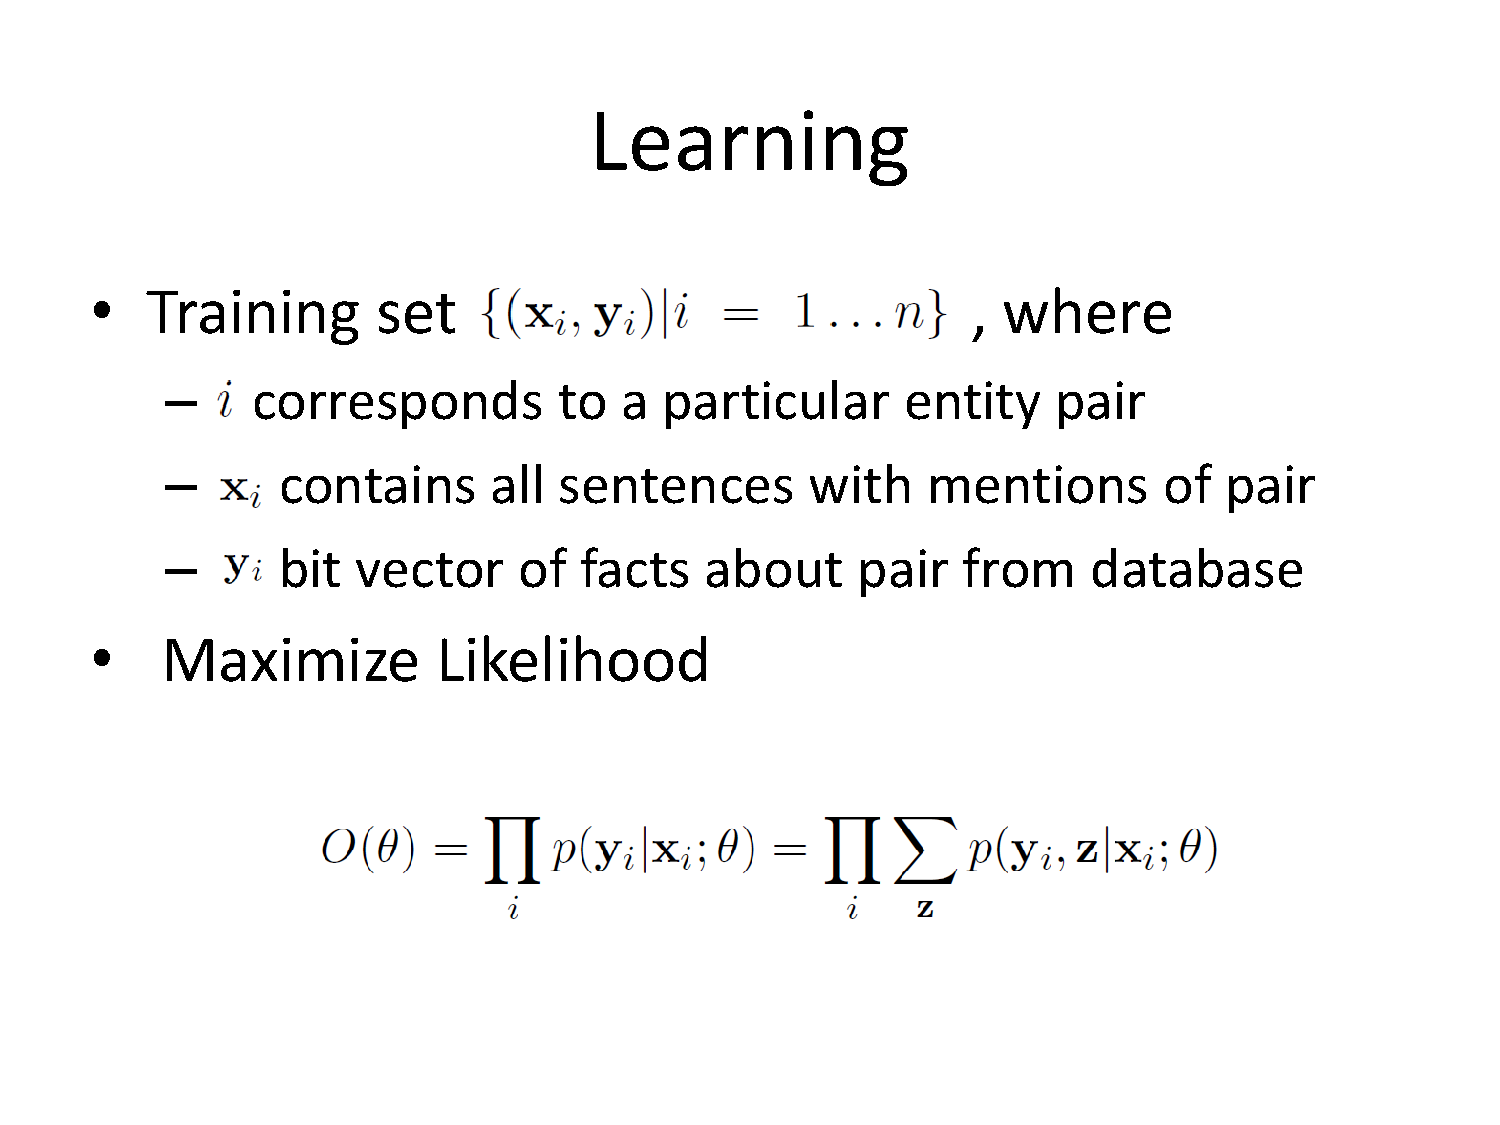
\includegraphics[scale=0.40]{./imgs/multirmode6.pdf}
 % multirmode.1.pdf: 720x540 pixel, 72dpi, 25.40x19.05 cm, bb=0 0 720 540
 \end{figure}
\end{frame}
\begin{frame}{Relation Extraction Using MultiR}{From \url{raphaelhoffmann.com/publications}}
\begin{figure}[h]
 \centering
 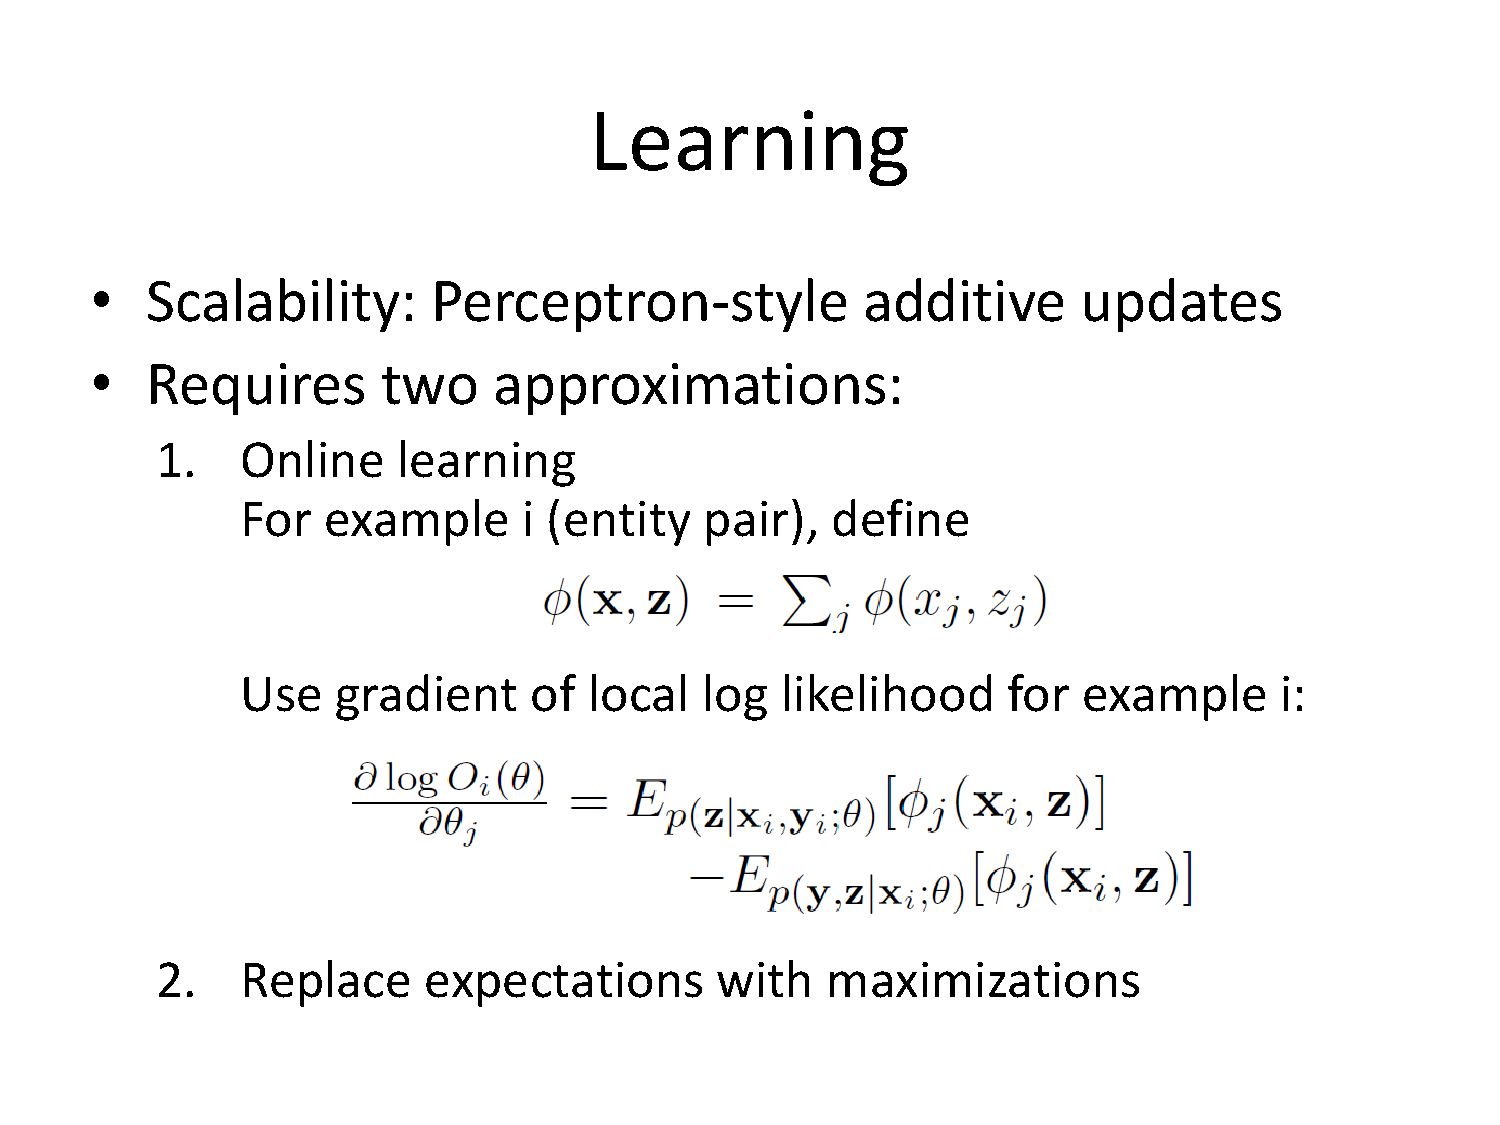
\includegraphics[scale=0.40]{./imgs/multirmode7.pdf}
 % multirmode.1.pdf: 720x540 pixel, 72dpi, 25.40x19.05 cm, bb=0 0 720 540
 \end{figure}
\end{frame}
\begin{frame}{Relation Extraction Using MultiR}{From \url{raphaelhoffmann.com/publications}}
\begin{figure}[h]
 \centering
 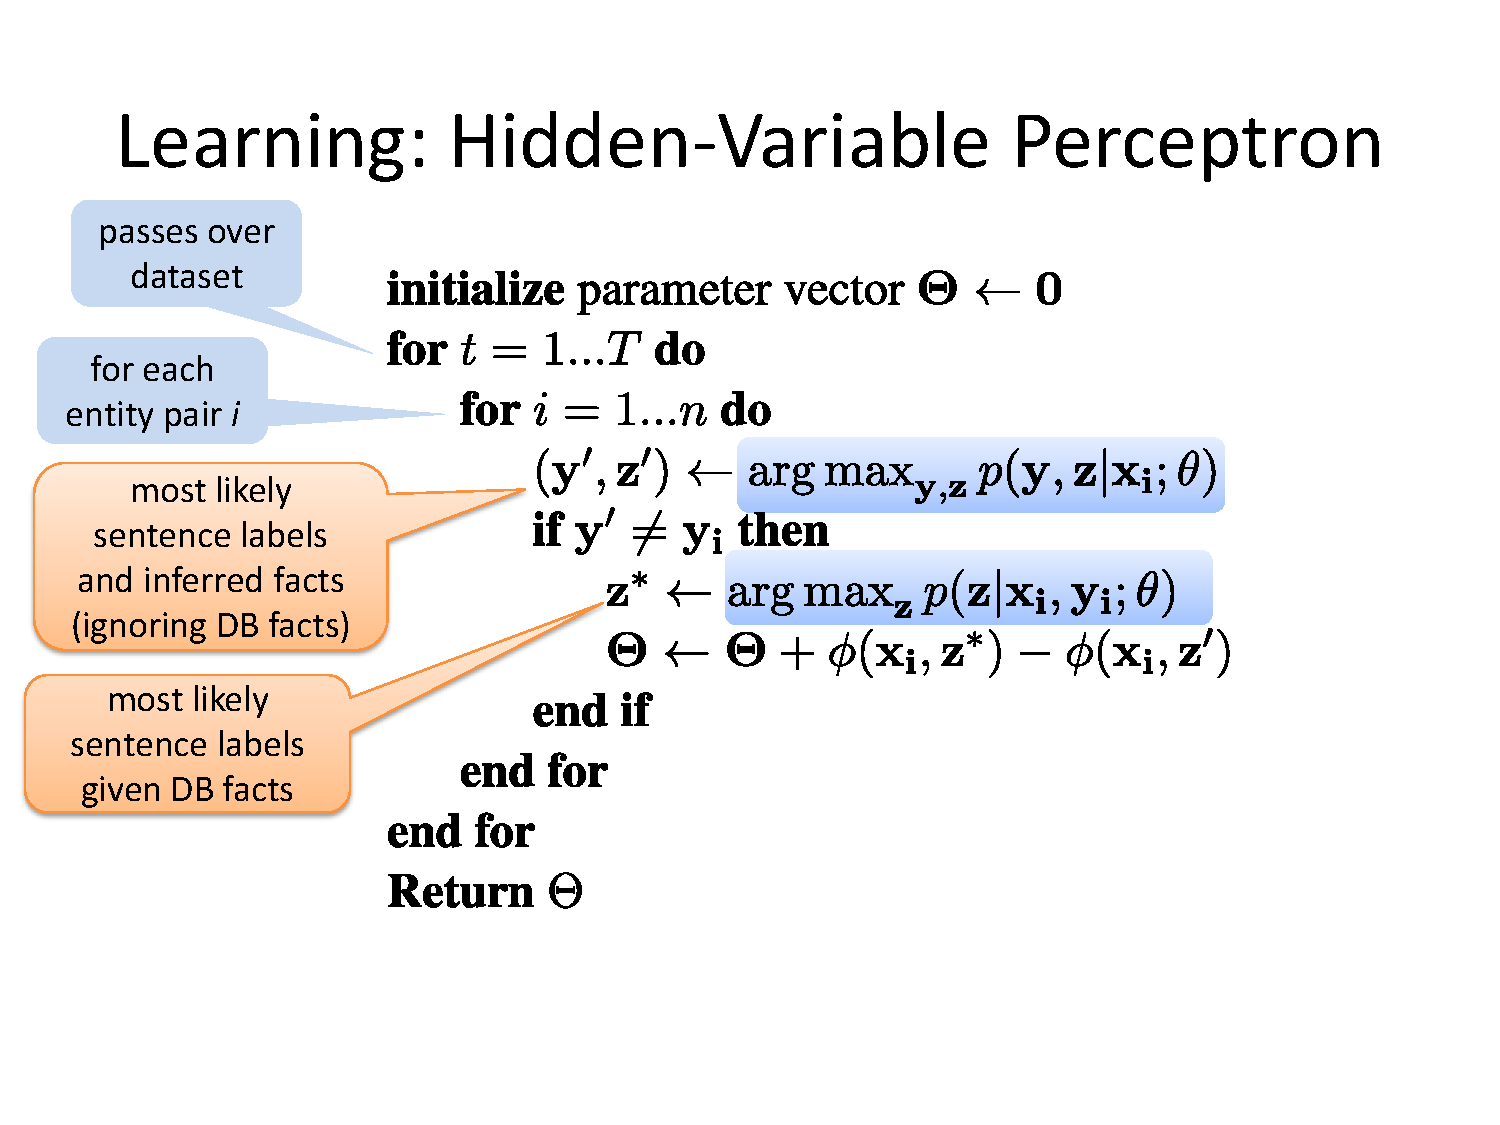
\includegraphics[scale=0.40]{./imgs/multirmode8.pdf}
 % multirmode.1.pdf: 720x540 pixel, 72dpi, 25.40x19.05 cm, bb=0 0 720 540
 \end{figure}
\end{frame}

% %PART 5: TAC Submission
\section{TAC Submission}
\begin{frame}{Cold Start Knowledge Base Population, 2014}
\begin{itemize}
 
 \item Knowledge Base Population (KBP) track of TAC encourages the development of systems that can match entities mentioned in natural texts with those
appearing in a knowledge base and extract novel information about entities from a document collection and add it to a new or existing knowledge base. \pause
 
 \item Some example relations:
    \begin{itemize}
      \item children of
      \item city of birth
      \item shareholders
      \item countries of residence
    \end{itemize}
\end{itemize}

\end{frame}
\begin{frame}{Cold Start Knowledge Base Population}

\begin{itemize}
  \item  Modeled the problem using distant supervision
  \item Used Freebase as an existing Knowledge base.
    
    \item \textbf{Freebase: }Freebase is a large collaborative knowledge base consisting of metadata composed mainly by its community members. 
    \item It is an online collection of structured data harvested from many sources, including individual, user-submitted wiki contributions.
 \end{itemize}

 
\end{frame}
\begin{frame}{Corpus}
 \begin{itemize}
  \item The TAC corpus consisted of three type of documents: \pause
    \begin{itemize}
	\item \textbf{discussion forums } 99,063 English discussion forum documents selected from the BOLT Phase 1 discussion forums source data releases. Each forum includes at least 5 posts. \pause

	\item \textbf{newswire } 1,000,257 documents selected from English Gigaword Fifth Edition. \pause

	 \item \textbf{web} 999,999 English web documents selected from various GALE web collections. \pause
    \end{itemize}
    
      \item We have submitted the knowledge base populated using our techniques on the above corpus and waiting for results.
 \end{itemize}


 
\end{frame}


\section{Numerical Relation Extraction}
%%THIS IS PART 6 : numerical relation extraction using distant supervision

\begin{frame}{Distant supervision for Numerical Relation Extraction}{Knowledge Base}
 \begin{itemize}
  \item Derived from \url{data.worldbank.org}, 4371979 numerical facts about 249 countries, 1281 attributes 

\begin{tabular}{|l|l|l|}
\hline
/m/04g5k&3126000130&EG.ELC.PROD.KH\\
/m/02k8k&1969.179&EN.ATM.CO2E.KT\\
/m/06nnj&332315&SP.POP.TOTL\\
/m/019rg5&55.020073&SP.DYN.LE00.IN\\
/m/05sb1&19974.148&EN.ATM.CO2E.KT\\
/m/05v8c&10000000000&EG.ELC.PROD.KH\\
/m/03spz&7639000100&EG.ELC.PROD.KH\\
/m/06vbd&44249.688&EN.ATM.CO2E.KT\\
/m/0d060g&51.3&IT.NET.USER.P2\\
/m/05qkp&62.298927&SP.DYN.LE00.IN\\
\hline
\end{tabular}


\end{itemize}

\end{frame}


\begin{frame}{Selected Relations}
 \begin{center}
\begin{tabular}{|l|l|}
\hline
Relation Name & Relation Code \\
\hline
Land area (sq. km)&AG.LND.TOTL.K2\\
Foreign direct investment, net (current US\$)&BN.KLT.DINV.CD\\
Goods exports (current US\$)&BX.GSR.MRCH.CD\\
Electricity production (kWh)&EG.ELC.PROD.KH\\
CO2 emissions (kt)&EN.ATM.CO2E.KT\\
Pump price for diesel fuel (US\$ per liter)&EP.PMP.DESL.CD\\
Inflation, consumer prices (annual \%)&FP.CPI.TOTL.ZG\\
Internet users (per 100 people)&IT.NET.USER.P2\\
GDP (current US\$)&NY.GDP.MKTP.CD\\
Life expectancy at birth, total (years)&SP.DYN.LE00.IN\\
Population (Total)&SP.POP.TOTL\\
\hline
\end{tabular}
\end{center}

\end{frame}
\begin{frame}{Corpus}
\begin{itemize}
 \item Subset of the tac corpus
 \item 268, 036 Documents, X sentences having a country and a number 
 \item List of countries augmented manually by adding all possible synonyms (Dutch, Netherlands) and inflections (Ireland, Irish)
\end{itemize}

 
\end{frame}
\begin{frame}{Distant supervision process for numerical relation extraction}
 \begin{itemize}
  \item Extract a country and number from a sentence, go to kb and check if there is a match.
  \item Can be creative during matching:
  \begin{itemize}
   \item Distance based matching
   \item Time based matching
  \end{itemize}
 \end{itemize}
\end{frame}
\begin{frame}{False Positives}{Numbers are weak entities}
\begin{itemize}
 \item Vanilla numerical relation matching is bound to attract humoungous amounts of false positives;
 \item Stems from the fact that numbers don't have an identity of their own.
 \item Consider {\SoulColor\hl{India}} and {\SoulColor\hl{Mumbai}} Vs. {\SoulColor\hl{India}} and {\SoulColor\hl{19}}
 \item {\SoulColor\hl{Mumbai}} is a strong entity, {\SoulColor\hl{19}} is a \textbf{weak} entity.
 \end{itemize}
\end{frame}
\begin{frame}{False Positives}{Numbers are weak entities}
 \begin{itemize}  
 \item Compare the number of sentences in which {\SoulColor\hl{India}} and {\SoulColor\hl{Mumbai}} appear together, vs the number of sentences
  in which {\SoulColor\hl{India}} and {\SoulColor\hl{19}} appear together.
 \item Just {\SoulColor\hl{19}} can be appear with India in several contexts:
 \begin{itemize}
 \item Internet user \%
 \item Billion dollars invested by a company
 \item \% of people below the poverty line
 \item date (if we are not careful)
 \item number of medals won by Indian athletes...
\end{itemize}

 \item Can we expect the situation to be even worse for certain types of numbers?
\end{itemize}
\end{frame}
\begin{frame}{One Thousand Words}
 \begin{center}
 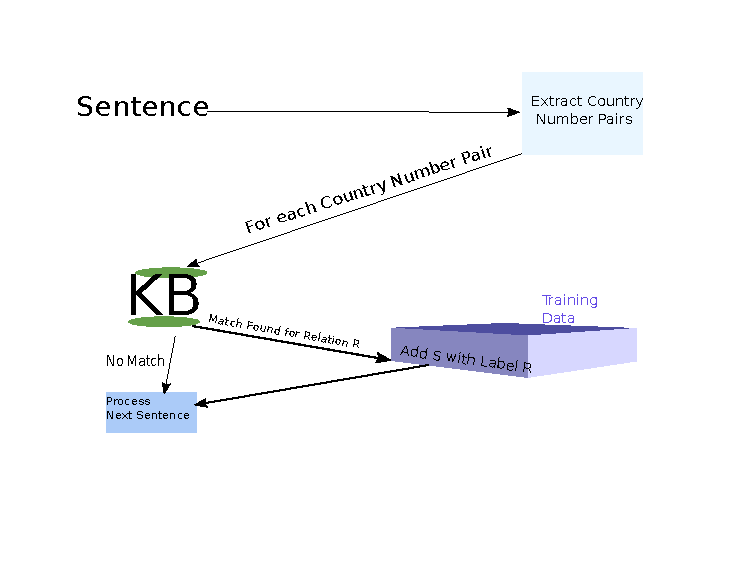
\includegraphics{./imgs/simple.pdf}
 % simple.pdf: 363x272 pixel, 72dpi, 12.81x9.60 cm, bb=0 0 363 272
\end{center}

\end{frame}

%PART 7 : Units
\section{Units in Numerical Relation Extraction}
\begin{frame}
 
 \frametitle{Numbers are incomplete without units} \pause
 
 \begin{itemize}
  
  \item  Apart from being a constant quantity, a number usually makes sense when presented along with units. \pause
  
    \begin{figure}
    \centering
    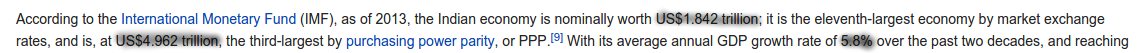
\includegraphics[width = 1.0\textwidth]{images/ex_6}
  \end{figure}
  \pause 
  \item Units help in improving recall.  \pause
  
  \begin{itemize}
      \item In above example 1.842 as number alone would not match with the fact regarding economy in knowledge base. \pause
      \item But with the unit trillion USD, we can normalize the value and then it would match exisiting facts in knowledge base. 
      
  \end{itemize}
  \end{itemize}
  \end{frame}

\begin{frame}
 
 \frametitle{Numbers are incomplete without units} \pause
 
 \begin{itemize}
  
  \item  Apart from being a constant quantity, a number usually makes sense when presented along with units. \pause
  
    \begin{figure}
    \centering
    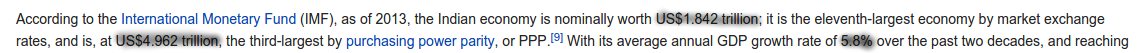
\includegraphics[width = 1.0\textwidth]{images/ex_6}
  \end{figure}
  \pause 
  \item Units help in improving recall.  \pause
  
  \begin{itemize}
      \item In above example 1.842 as number alone would not match with the fact regarding economy in knowledge base. \pause
      \item But with the unit trillion USD, we can normalize the value and then it would match exisiting facts in knowledge base. 
      
  \end{itemize}
  \end{itemize}
  \end{frame}
  
\begin{frame}
  \frametitle{Numbers are incomplete without units} 
    \begin{figure}
    \centering
    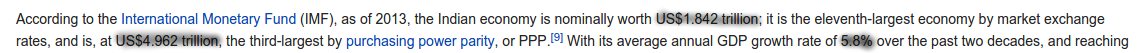
\includegraphics[width = 1.0\textwidth]{images/ex_6}
  \end{figure}
  
  \begin{itemize}
  \item Units help in reducing false positives and hence improving precision. \pause
  \begin{itemize}
      \item If there is a fact, e.g, \textbf{inflation(India, 1.842\%)} in knowledge base, then ignoring units can cause an incorrect match which leads in learning towards noisy patterns.
  \end{itemize}
  
 \end{itemize}

 
\end{frame}

\begin{frame}
 \frametitle{Unit Extraction is not easy!} \pause
 
 \begin{itemize}
    \item Different ways to represent a single unit. \pause
    
    \begin{itemize}
     \item Tunisia occupies an area of 163,610 \textbf{square kilometres}, of which 8,250 are water. \pause
     \item With an area of about 9.6 \textbf{million $km^{2}$}, the People's Republic of China is the 3rd largest country in total area behind Russia and Canada, and very similar to the United States.
    \end{itemize}
\pause
    
    \item Multiple units to represent a single numerical fact. \pause
    \begin{itemize}
      \item Vatican City, a walled enclave within the city of Rome, with an area of approximately \textbf{44 hectares} \textbf{(110 acres)}, and a population of 842, is the smallest internationally recognized independent state in the world by both area and population.
    \end{itemize}
 \end{itemize}
\end{frame}


\begin{frame}
 \frametitle{Overview of Unit Extraction System} \pause
 
 \begin{itemize}
  
  \item A discriminative context free grammmar with scores
attached to each possible production in the grammar. \pause
  \item A production P in the grammar is of the form  $ R ::= R_{1} R_{2}$ , scored as 
\begin{equation*}
	score(P) = \textbf{w . f}(P, x, i, j, k), 
\end{equation*}
where $(i,j)$ and $(j+1,k)$ are text spans in $x$ that $R_{1}$ and $R_{2}$
cover.
 \end{itemize}
\end{frame}

\begin{frame}
 \frametitle{Overview of Unit Extraction System}
 \begin{itemize}
  \item Some of the features that grammar uses to assign the best scores to various
parses are as belows: \pause
    \begin{itemize}
        \item Matches with Unit Catalog \pause
	\item Lexical Clues \pause
	\item Relative Frequency - Prior of the word to be present as unit, then as an
	  non-unit word. This is derived from WordNet ontologies. \pause
	\item Co-occurrence statistics - presence of strongly co-occuring words in the
	  text can help in disambiguating the various candidate units 
    \end{itemize}
 \end{itemize}


    \begin{figure}
    \centering
    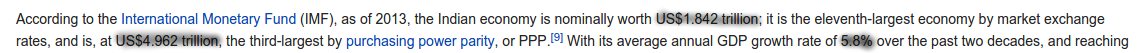
\includegraphics[width = 1.0\textwidth]{images/ex_6}
  \end{figure}
  
  \begin{itemize}
  \item Units help in reducing false positives and hence improving precision. \pause
  \begin{itemize}
      \item If there is a fact, e.g, \textbf{inflation(India, 1.842\%)} in knowledge base, then ignoring units can cause an incorrect match which leads in learning towards noisy patterns.
  \end{itemize}
  
 \end{itemize}

 
\end{frame}
\begin{frame}
 \frametitle{Unit Extraction is not easy!} \pause
 
 \begin{itemize}
    \item Different ways to represent a single unit. \pause
    
    \begin{itemize}
     \item Tunisia occupies an area of 163,610 \textbf{square kilometres}, of which 8,250 are water. \pause
     \item With an area of about 9.6 \textbf{million $km^{2}$}, the People's Republic of China is the 3rd largest country in total area behind Russia and Canada, and very similar to the United States.
    \end{itemize}
\pause
    
    \item Multiple units to represent a single numerical fact. \pause
    \begin{itemize}
      \item Vatican City, a walled enclave within the city of Rome, with an area of approximately \textbf{44 hectares} \textbf{(110 acres)}, and a population of 842, is the smallest internationally recognized independent state in the world by both area and population.
    \end{itemize}
 \end{itemize}
\end{frame}
\begin{frame}
 \frametitle{Overview of Unit Extraction System} \pause
 
 \begin{itemize}
  
  \item A discriminative context free grammmar with scores
attached to each possible production in the grammar. \pause
  \item A production P in the grammar is of the form  $ R ::= R_{1} R_{2}$ , scored as 
\begin{equation*}
	score(P) = \textbf{w . f}(P, x, i, j, k), 
\end{equation*}
where $(i,j)$ and $(j+1,k)$ are text spans in $x$ that $R_{1}$ and $R_{2}$
cover.
 \end{itemize}
\end{frame}
\begin{frame}
 \frametitle{Overview of Unit Extraction System}
 \begin{itemize}
  \item Some of the features that grammar uses to assign the best scores to various
parses are as belows: \pause
    \begin{itemize}
        \item Matches with Unit Catalog \pause
	\item Lexical Clues \pause
	\item Relative Frequency - Prior of the word to be present as unit, then as an
	  non-unit word. This is derived from WordNet ontologies. \pause
	\item Co-occurrence statistics - presence of strongly co-occuring words in the
	  text can help in disambiguating the various candidate units 
    \end{itemize}
 \end{itemize}

 
 
\end{frame}

%PART 8 : Keywords
\begin{frame}{A case for Keywords}
 \begin{itemize}
  \item A large number of false matches had no reference to the relation involved.
  \item Eg. No mention of Population in the following matches:
  \begin{itemize}
  \item The website of \SoulColor\hl{China's} Ministry of Defense (MOD) has attracted around \SoulColor\hl{1.25} billion visits in the three months since its opening, with the United States topping the source countries for foreign visits, website editor-in-chief Ji Guilin said.
  \item Insulza, for his part, said the Organization of American States expects to raise \SoulColor\hl{10 million} dollars for \SoulColor\hl{Haiti's} recovery.
  \item Koloini and others brought 10 million euros, probably \SoulColor\hl{15 million}, back from \SoulColor\hl{Iraq} at the time, Falter quoted from the diary.
 \end{itemize}
\item No reference to Co2 emission:
 \begin{itemize}
 \item \SoulColor\hl{China's} iron ore imports surged 41.6 percent to \SoulColor\hl{627.8 million tonnes} in 2009, with the value falling 17.4 percent as prices were hit by the global downturn, customs data shows.
 \end{itemize}
 \end{itemize}

\end{frame}
\begin{frame}{A case for Keywords}
 \begin{exampleblock}{Good News}
  Sentences expressing a numerical relation can be expected to have keywords that denote the relation
 \end{exampleblock}

 \begin{itemize}
  \item Take all the labeled sentences, prune out sentences that don't have atleast one of the relevant keywords
 \end{itemize}
 
 \begin{tabular}{|l|l|}
  \hline
  Internet User \% & "Internet" \\
Land Area & "area", "land", "land area" \\
Population &"Population" \\
Diesel & "diesel" \\
GDP &"Gross domestic", "GDP" \\
CO2 &"Carbon", "Carbon Emission", "CO2" \\
Inflation & "Inflation", "Price Rise" \\
FDI & "Foreign", "FDI" \\
Goods Export & "goods" \\
Life Expectancy & "life", "life expectancy" \\
Electricity Production & "Electricity" \\
 \hline
 \end{tabular}
\end{frame}
\begin{frame}{A case for Keywords}
\begin{itemize}
  \item Numbers are the second entity in our setup (Relation(Country, Number))
  \item Unlike real world entities, numbers don't have an identity of their own, sentences should have words (keywords!) indicating what the number stands for
  \item Manual inspection of 400 sentences pruned out after applying keyword based filter backs this conjecture, not even one false negative
  \item The keywords are created manually, can this process be automated?
\end{itemize}
\end{frame}
\section{Results}

\end{document}

